%
% ---------------------------------------------------------------
% Copyright (C) 2012-2018 Gang Li
% ---------------------------------------------------------------
%
% This work is the default powerdot-tuliplab style test file and may be
% distributed and/or modified under the conditions of the LaTeX Project Public
% License, either version 1.3 of this license or (at your option) any later
% version. The latest version of this license is in
% http://www.latex-project.org/lppl.txt and version 1.3 or later is part of all
% distributions of LaTeX version 2003/12/01 or later.
%
% This work has the LPPL maintenance status "maintained".
%
% This Current Maintainer of this work is Gang Li.
%
%

\documentclass[
 size=14pt,
 paper=smartboard,  %a4paper, smartboard, screen
 mode=present, 		%present, handout, print
 display=slides, 	% slidesnotes, notes, slides
 style=tuliplab,  	% TULIP Lab style
 pauseslide,
 fleqn,leqno]{powerdot}


\usepackage{cancel}
\usepackage{caption}
\usepackage{stackengine}
\usepackage{smartdiagram}
\usepackage{attrib}
\usepackage{amssymb}
\usepackage{amsmath} 
\usepackage{amsthm} 
\usepackage{mathtools}
\usepackage{rotating}
\usepackage{graphicx}
\usepackage{boxedminipage}
\usepackage{rotate}
\usepackage{calc}
\usepackage[absolute]{textpos}
\usepackage{psfrag,overpic}
\usepackage{fouriernc}
\usepackage{pstricks,pst-3d,pst-grad,pstricks-add,pst-text,pst-node,pst-tree}
\usepackage{moreverb,epsfig,subfigure}
\usepackage{color}
\usepackage{booktabs}
\usepackage{etex}
\usepackage{breqn}
\usepackage{multirow}
\usepackage{natbib}
\usepackage{bibentry}
\usepackage{gitinfo2}
\usepackage{siunitx}
\usepackage{nicefrac}
%\usepackage{geometry}
%\geometry{verbose,letterpaper}
\usepackage{media9}
\usepackage{animate}
%\usepackage{movie15}
\usepackage{auto-pst-pdf}

\usepackage{breakurl}
\usepackage{fontawesome}
\usepackage{xcolor}
\usepackage{multicol}



\usepackage{verbatim}
\usepackage[utf8]{inputenc}
\usepackage{dtk-logos}
\usepackage{tikz}
\usepackage{adigraph}
%\usepackage{tkz-graph}
\usepackage{hyperref}
%\usepackage{ulem}
\usepackage{pgfplots}
\usepackage{verbatim}
\usepackage{fontawesome}


\usepackage{todonotes}
% \usepackage{pst-rel-points}
\usepackage{animate}
\usepackage{fontawesome}

\usepackage{listings}
\lstset{frameround=fttt,
frame=trBL,
stringstyle=\ttfamily,
backgroundcolor=\color{yellow!20},
basicstyle=\footnotesize\ttfamily}
\lstnewenvironment{code}{
\lstset{frame=single,escapeinside=`',
backgroundcolor=\color{yellow!20},
basicstyle=\footnotesize\ttfamily}
}{}


\usepackage{hyperref}
\hypersetup{ % TODO: PDF meta Data
  pdftitle={Presentation Title},
  pdfauthor={Gang Li},
  pdfpagemode={FullScreen},
  pdfborder={0 0 0}
}


% \usepackage{auto-pst-pdf}
% package to show source code

\definecolor{LightGray}{rgb}{0.9,0.9,0.9}
\newlength{\pixel}\setlength\pixel{0.000714285714\slidewidth}
\setlength{\TPHorizModule}{\slidewidth}
\setlength{\TPVertModule}{\slideheight}
\newcommand\highlight[1]{\fbox{#1}}
\newcommand\icite[1]{{\footnotesize [#1]}}

\newcommand\twotonebox[2]{\fcolorbox{pdcolor2}{pdcolor2}
{#1\vphantom{#2}}\fcolorbox{pdcolor2}{white}{#2\vphantom{#1}}}
\newcommand\twotoneboxo[2]{\fcolorbox{pdcolor2}{pdcolor2}
{#1}\fcolorbox{pdcolor2}{white}{#2}}
\newcommand\vpspace[1]{\vphantom{\vspace{#1}}}
\newcommand\hpspace[1]{\hphantom{\hspace{#1}}}
\newcommand\COMMENT[1]{}

\newcommand\placepos[3]{\hbox to\z@{\kern#1
        \raisebox{-#2}[\z@][\z@]{#3}\hss}\ignorespaces}

\renewcommand{\baselinestretch}{1.2}


\newcommand{\draftnote}[3]{
	\todo[author=#2,color=#1!30,size=\footnotesize]{\textsf{#3}}	}
% TODO: add yourself here:
%
\newcommand{\gangli}[1]{\draftnote{blue}{GLi:}{#1}}
\newcommand{\shaoni}[1]{\draftnote{green}{sn:}{#1}}
\newcommand{\gliMarker}
	{\todo[author=GLi,size=\tiny,inline,color=blue!40]
	{Gang Li has worked up to here.}}
\newcommand{\snMarker}
	{\todo[author=Sn,size=\tiny,inline,color=green!40]
	{Shaoni has worked up to here.}}

%%%%%%%%%%%%%%%%%%%%%%%%%%%%%%%%%%%%%%%%%%%%%%%%%%%%%%%%%%%%%%%%%%%%%%%%
% title
% TODO: Customize to your Own Title, Name, Address
%
\title{New York City Taxi Trip Duration Prediction}
\author{
Weiling Deng
\\
\\Deakin University
}
\date{\gitCommitterDate}


% Customize the setting of slides
\pdsetup{
% TODO: Customize the left footer, and right footer
rf=\href{http://www.tulip.org.au}{
Last Changed by: \textsc{\gitCommitterName}\ \gitVtagn-\gitAbbrevHash\ (\gitAuthorDate)
},
cf={New York City Taxi Trip Duration Prediction},
}


\begin{document}

\maketitle

%\begin{slide}{Overview}
%\tableofcontents[content=sections]
%\end{slide}


%%==========================================================================================
%%
\begin{slide}[toc=,bm=]{Overview}
\tableofcontents[content=currentsection,type=1]
\end{slide}
%%
%%==========================================================================================


\section{Problem Definition}


%%==========================================================================================
%%
\begin{slide}{New York City Taxi Trip Duration Prediction}
\begin{center}
\twotonebox{\rotatebox{90}{Defn}}{\parbox{.86\textwidth}
{New York City Taxi Trip Duration Prediction aims to
identify the outstanding features of the query object.
\begin{itemize}
\item We may be interested in the \textcolor{orange}{characteristics} that
make \textcolor{orange}{distance} \textcolor{orange}{trip duration} .
\item How the relationship between the distance and tripduration, and we use distance to predict trip duration (a query object).
\end{itemize}
}}

\end{center}

\bigskip


%%==========================================================================================

\end{slide}
%%
%%==========================================================================================


\section{Data ETL}


%%==========================================================================================
%%
\begin{slide}{Data ETL - Data Loading}
%Data ETL - Data Loading
\begin{itemize}
\item
Data Loading - \textcolor{orange}{import data from csv files}

\begin{itemize}
\item
There are train data and test data:
\end{itemize}
\vspace{1cm}
\twocolumn[
\savevalue{lfrheight}=5cm,
\savevalue{lfrprop}={
linestyle=solid,framearc=.2,linewidth=1pt},
rfrheight=\usevalue{lfrheight},
rfrprop=\usevalue{lfrprop}
]{
Train Data
\begin{itemize}
\item
\smallskip
Name test data as df\_train data

\item
\smallskip
There are \textcolor{orange}{1458644} Rows and \textcolor{orange}{11} columns.

\item
\smallskip
\end{itemize}
}
{
Test Data
\begin{itemize}
\item
\smallskip
Name test data as df\_test data

\item
\smallskip
There are \textcolor{orange}{625134} Rows and \textcolor{orange}{9} columns.
\end{itemize}
}
\end{itemize}

%%==========================================================================================

%%==========================================================================================

\end{slide}
%%
%%==========================================================================================



%%==========================================================================================
%%
\begin{slide}{Read Data and Print out}
	%Data Loading-- Print Train and Test Data
	{\begin{flushleft}
			\includegraphics[width=0.98\textwidth]{figures/pe.eps}
		\end{flushleft}
	}
\end{slide}
%%
%%==============================================================================




%%==========================================================================================
%%
\begin{slide}{Data Clean and check NA}
	\twocolumn[lcolwidth=0.45\linewidth,
	rcolwidth=0.45\linewidth
	]{
		\begin{flushleft}
			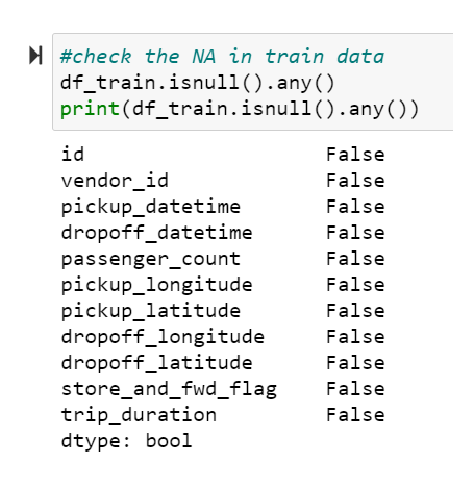
\includegraphics[width=0.8\textwidth]{figures/pe2.eps}
	\end{flushleft}}
	{\begin{flushleft}
			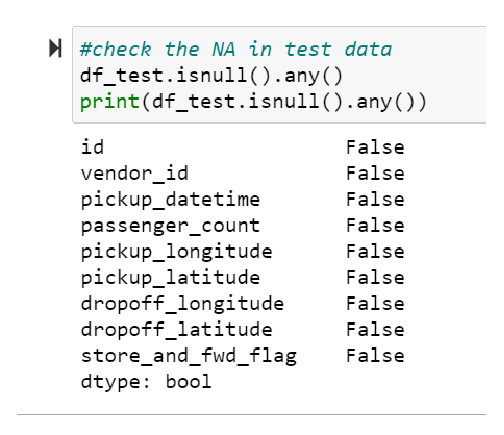
\includegraphics[width=0.8\textwidth]{figures/pe3.eps}
		\end{flushleft}
	}

\begin{itemize}
	\item
	\smallskip
	Clean Data and check NA, the result shows that there is no NA 
	
\end{itemize}

\end{slide}
%%
%%===============================================================================



%%==========================================================================================
%%
\begin{slide}{Data Discrible}
	\twocolumn[lcolwidth=0.45\linewidth,
	rcolwidth=0.45\linewidth
	]{
		\begin{flushleft}
			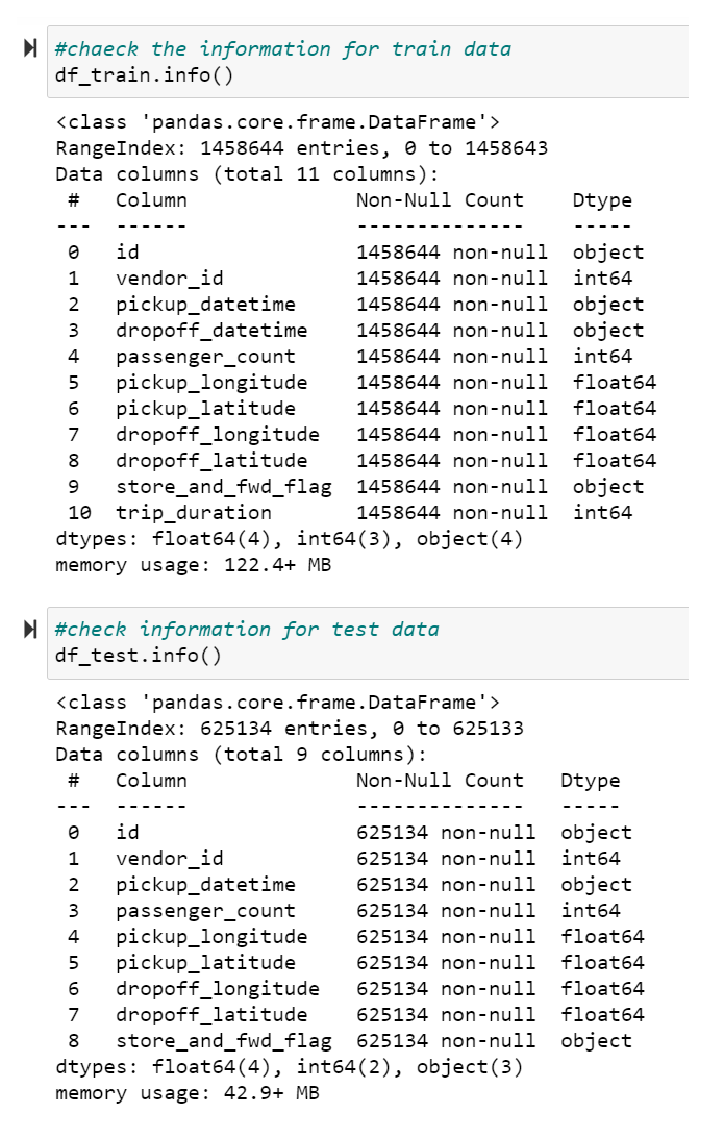
\includegraphics[width=0.8\textwidth]{figures/pe4.eps}
	\end{flushleft}}
	{\begin{flushleft}
			\includegraphics[width=0.8\textwidth]{figures/pe5.eps}
		\end{flushleft}
	}
\end{slide}
%%
%%===============================================================================

%%==========================================================================================


\section{Knowledge Discovery}


%%==========================================================================================


%%==========================================================================================
%%
\begin{slide}{Calculate the distance by latitude and longitude}
	{\begin{flushleft}
			\includegraphics[width=0.75\textwidth]{figures/pe6.eps}
		\end{flushleft}
	}
\end{slide}
%%
%%==============================================================================




%%==========================================================================================
%%
\begin{slide}{Data Visualization- Distribution distance}
	\twocolumn[lcolwidth=0.5\linewidth,
rcolwidth=0.5\linewidth
]{
	\begin{flushleft}
		\includegraphics[width=0.8\textwidth]{figures/pe7.eps}
\end{flushleft}}
{\begin{flushleft}
		\includegraphics[width=0.8\textwidth]{figures/pe8.eps}
	\end{flushleft}
}

\begin{itemize}
	\item
	\smallskip
	Distribution distance and visualization the data in train data and test data as well, try to find some features with these data.

\end{itemize}
	
\end{slide}
%%
%%==============================================================================


%%==========================================================================================
%%
\begin{slide}{Distribution Trip Duration and Visualization}
	{\begin{flushleft}
			\includegraphics[width=0.78\textwidth]{figures/pe9.eps}
		\end{flushleft}
	}

\begin{itemize}
	\item
	\smallskip
	Distribution trip duration and visualization the data in train data, try to find some features with these data.
	
\end{itemize}

\end{slide}
%%
%%==============================================================================




%%==========================================================================================
%%
\begin{slide}{Visualization Distance with Date and Trip Duration}
	\twocolumn[lcolwidth=0.55\linewidth,
	rcolwidth=0.55\linewidth
	]{
		\begin{flushleft}
			\includegraphics[width=0.8\textwidth]{figures/pe10.eps}
	\end{flushleft}}
	{\begin{flushleft}
			\includegraphics[width=0.8\textwidth]{figures/pe11.eps}
		\end{flushleft}
	}

\begin{itemize}
	\item
	\smallskip
	Visualization Distance with Date and Trip Duration, try to find some features with these data.
	
\end{itemize}

\end{slide}
%%
%%==============================================================================


%%==========================================================================================


\section{Model Built and Prediction}

%%==========================================================================================






%%==========================================================================================
%%
\begin{slide}{Select features and gropby data to train data and test data}
	\twocolumn[lcolwidth=0.45\linewidth,
	rcolwidth=0.45\linewidth
	]{
		\begin{flushleft}
			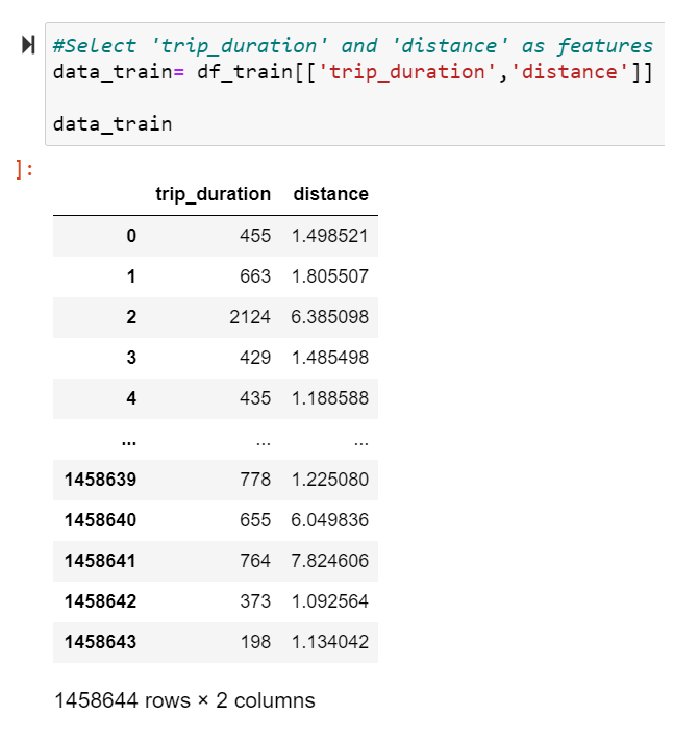
\includegraphics[width=0.8\textwidth]{figures/pe12.eps}
	\end{flushleft}}
	{\begin{flushleft}
			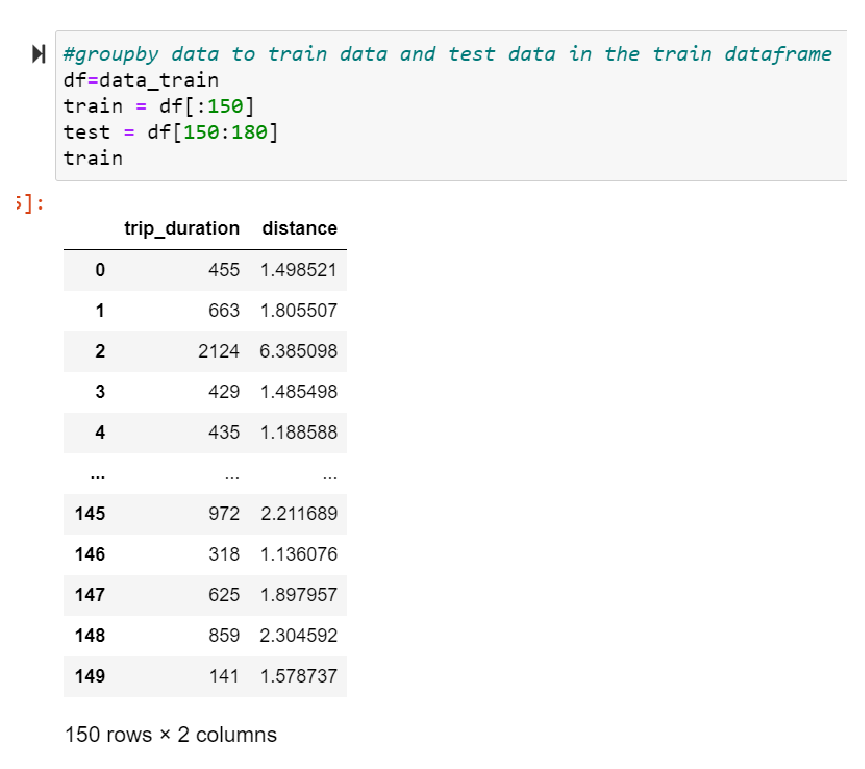
\includegraphics[width=0.8\textwidth]{figures/pe13.eps}
		\end{flushleft}
	}
	
	\begin{itemize}
		\item
		\smallskip
		Select 'trip duration' and 'distance' as features, groupby data to train data and test data in the train dataframe, set 0 to 150 as train data, 150 to 180 as test data, named as train and test.
		
	\end{itemize}
	
\end{slide}
%%
%%==============================================================================


%%==========================================================================================
%%
\begin{slide}{Built LinearRegresion Model and find best parameter to predict }
	{\begin{flushleft}
		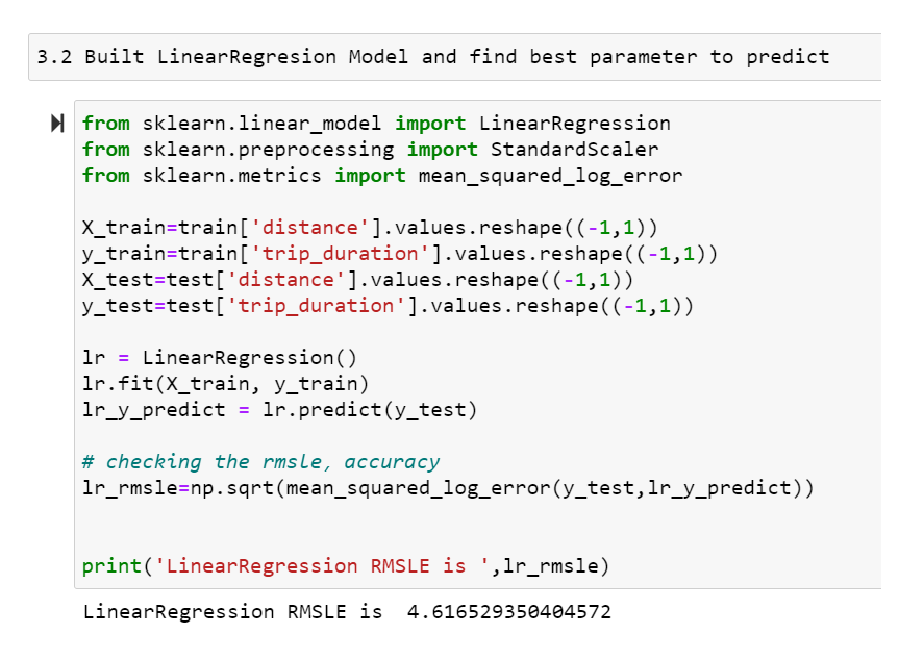
\includegraphics[width=0.5\textwidth]{figures/pe14.eps}
	\end{flushleft}
}
	
	\begin{itemize}
		\item
		\smallskip
		Built LinearRegresion Model and find best parameter to predict, we use distance to predict the trip duration and test. The result presents that the LinearRegression RMSLE is  4.616529350404572. 
		
	\end{itemize}
	
\end{slide}
%%
%%==============================================================================


%%==========================================================================================
%%
\begin{slide}{Visualization the predict data}
	{\begin{flushleft}
			\includegraphics[width=0.65\textwidth]{figures/pe15.eps}
		\end{flushleft}
	}
	
	\begin{itemize}
		\item
		\smallskip
		Visualization the predict data.
		
	\end{itemize}
	
\end{slide}
%%
%%==============================================================================



%%==========================================================================================


\section{Conclusion}

%%==========================================================================================
%%
\begin{slide}[toc=,bm=]{Conclusion}
\begin{itemize}
\item
\smallskip
Formalize the problem of \emph{New York City Taxi Trip Duration Prediction} 

\item
\smallskip
Propose to find the data features, select the attruibuates to built the linearregression model, find the best parameter using distance data to predict the trip duration and test.But , from the chart we can see the model is not very good, maybe we an explore other model to improve the accuracy.

\item
\smallskip
Utilize 

\end{itemize}

%%==========================================================================================

%%==========================================================================================

\end{slide}
%%
%%==========================================================================================
% TODO: Contact Page
\begin{wideslide}[toc=,bm=]{Contact Information}
\centering
\vspace{\stretch{1}}
\twocolumn[
lcolwidth=0.35\linewidth,
rcolwidth=0.65\linewidth
]
{
% \centerline{
\includegraphics[scale=.2]{tulip-logo.eps}}
}
{
\vspace{\stretch{1}}
Weiling Deng\\
Business School\\
Deakin University, Australia
\begin{description}
 \item[\textcolor{orange}{\faEnvelope}] \href{ddengpp@gmail.com}
 {\textsc{\footnotesize{ddengpp@gmail.com}}}

 \item[\textcolor{orange}{\faHome}] \href{http://www.tulip.org.au}
 {\textsc{\footnotesize{Team for FLIP00}}}
\end{description}
}
\vspace{\stretch{1}}
\end{wideslide}

\end{document}

\endinput
